\documentclass[10pt,a4paper,twoside,fleqn]{article}
\usepackage[left=25mm, top=20mm, bottom=20mm, right=20mm]{geometry}
\usepackage[utf8]{inputenc}
\usepackage[T1]{fontenc}
\usepackage[ngerman]{babel}	
\usepackage{amsmath}
\usepackage{amssymb,multicol,overpic}
\usepackage{cancel}
\usepackage {picins}
\usepackage{graphicx}
\usepackage{float}
\usepackage{icomma} 


\newcommand{\Vektor}[2]{\begin{pmatrix} #1 \\ #2 \end{pmatrix}}
\newcommand{\vektor}[3] {\begin{pmatrix} #1 \\ #2 \\ #3 \end{pmatrix}}

\renewcommand{\labelitemi}{\textbf{\alph{itemi}.)}}
\renewcommand{\labelenumi}{\textbf{\arabic{enumi}.)}}
\renewcommand{\labelenumii}{\textbf{\alph{enumi}.)}}
\setlength{\parindent}{0pt}

\begin{document}
	\author{} \date{}
	\title{Gegenseitige Lage von Objekten in vektorieller Darstellung}
	\maketitle
	


		\section{Punkt und Gerade}
		\subsection{Vorwissen}
			Ein Punkt wird in vektorieller Darstellung als Ortsvektor angegeben. Ein Ortsvektor ist der Vektor zu einem Punkt, der von Ursprung genau zu diesem Punkt führt. Zum Punkt X würde er mit einem Kleinbuchstaben $\vec{x}$ oder als Vektor $\vec{OX}$ benannt. 
			\text{Beispiel}
			Der Ortsvektor von $$ A(1|2|3) \qquad \text{ist} \qquad \vec{OA}=\vec{a}=\vektor{1}{2}{3}$$
			
			
			Eine Gerade wird in vektorieller Darstellung mithilfe zweier Komponenten angegeben: dem Richtungsvektor und dem Stützvektor. Der Richtungsvektor bestimmt die Richtung und wird mithilfe eines Parameters, der mit diesem multipliziert wird, gestreckt und gestaucht. Der Stützvektor schiebt die Gerade vom Ursprung weg, sodass sie überall beginnen kann. Man kann jede Gerade in dieser Parameterdarstellung angeben: $$\vec{x} = \text{Richtungsvektor} + r \cdot \text{Stützvektor}$$ \\
		\bigskip
			In dem Fall der Abbildung unten ist der Stützvektor $\Vektor{2}{3}$ und der Richtungsvektor $\Vektor{-3}{1}$. \\ Die Geradengleichung dieser Geraden heißt also $\vec{x}=\Vektor{2}{3} + r\cdot\Vektor{-3}{1}$\\
			\medskip
			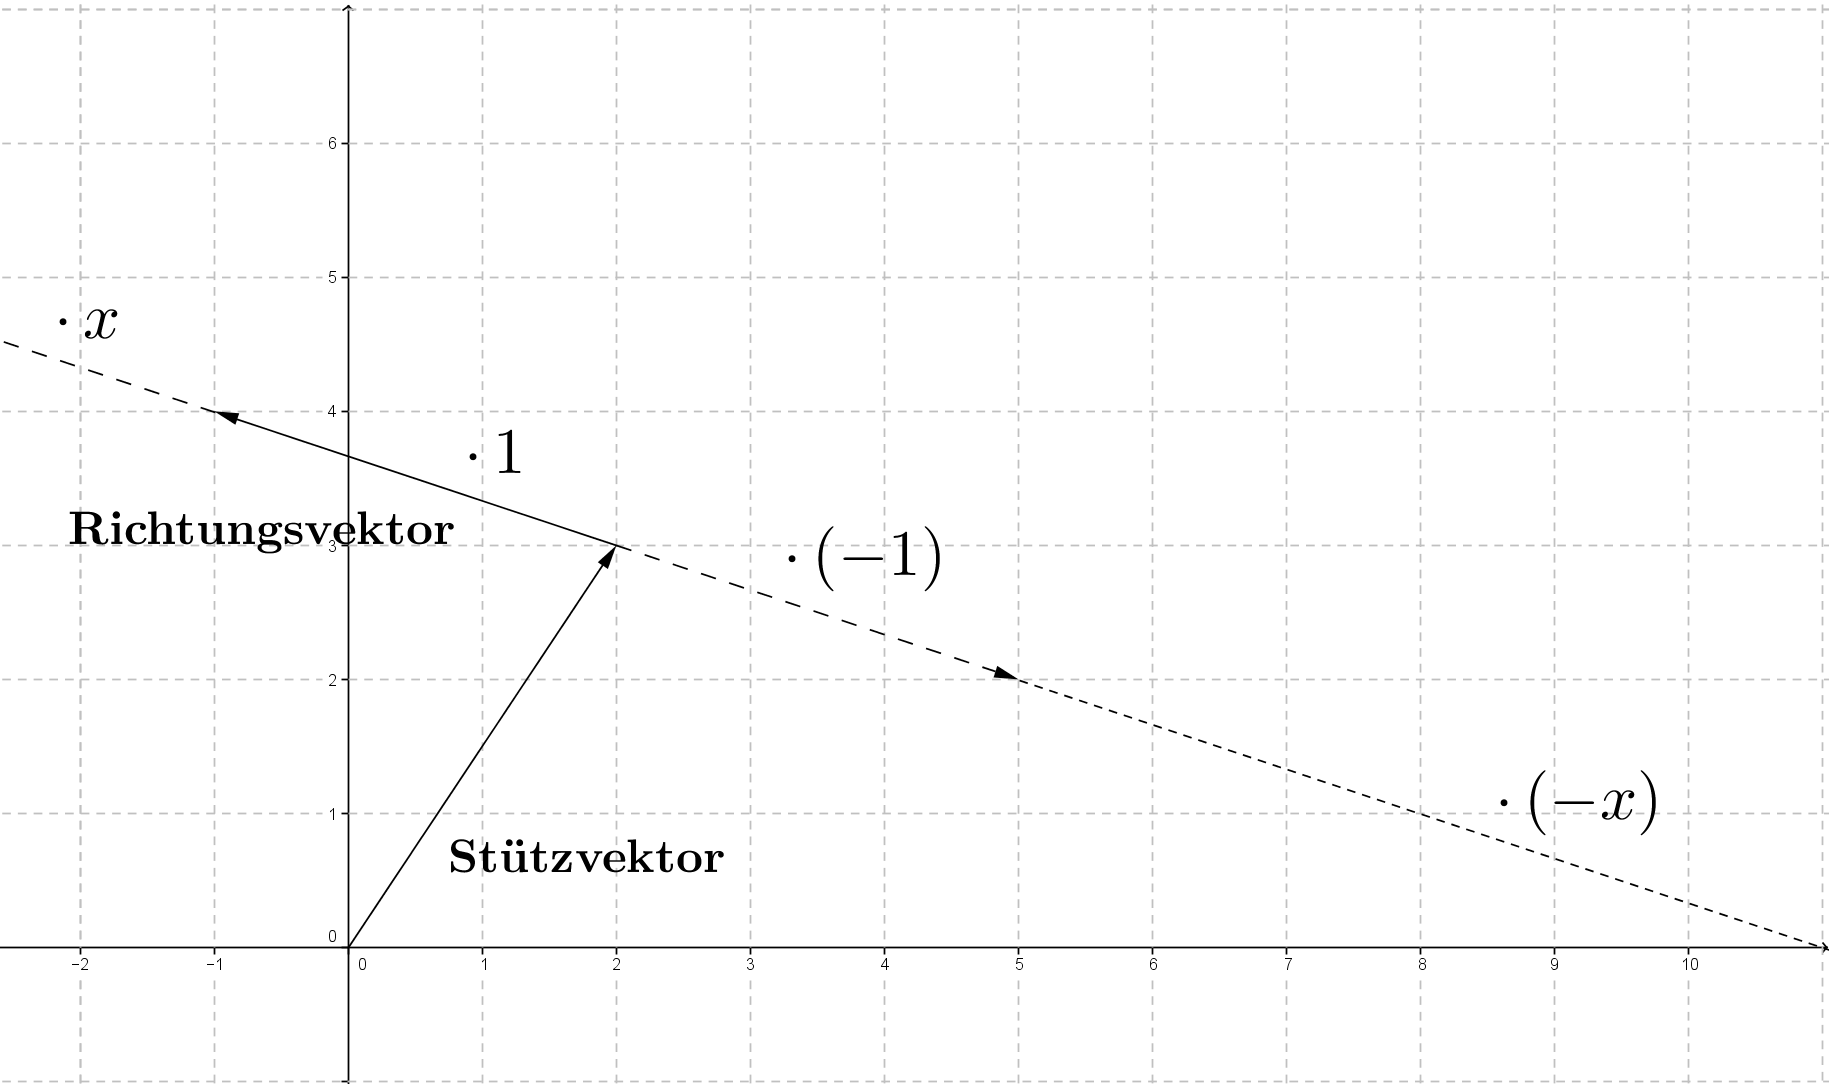
\includegraphics[keepaspectratio,width=\linewidth]{Gerade.png}
		\newpage		
		\subsection{Gegenseitige Lage}
			Ein Punkt und eine Gerade können nur zwei Mögliche Lagen zueinander haben. Entweder ist der Punkt ein Teil der Geraden oder er liegt daneben. Um zu Überprüfen, ob ein Punkt auf einer Geraden liegt, setzen wir den Punkt einfach als Lösung der Geraden ein.\\
			Wir überprüfen in einem Beispiel, ob der Punkt A(-4|5) auf der Geraden liegt:
			$$\Vektor{-4}{5}=\Vektor{2}{3} + r\cdot\Vektor{-3}{1}\qquad \left|-\Vektor{2}{3}\right.$$
			$$\Vektor{-6}{2} = r \cdot \Vektor{-3}{1} $$
		\medskip	
		
			An dieser Stelle können wir überprüfen, was für r eingesetzt werden muss, damit die $x_1$-Koordinate (die oberste Vektoren Zeile) stimmt:
			
			$$x_1 \rightarrow -6=r\cdot(-3) \quad \left|:(-3)\right. $$
			$$2=r$$
			Nun überprüfen wir, ob das für die andern Koordinaten auch stimmt:
			$$x_2-Probe \rightarrow\quad 2 = 2 \cdot 1 $$ 
			Da es ein r gibt, mit welchem die Gleichung lösbar ist, liegt der Punkt auf der Gerade. Sollte die Gleichung nicht zu lösen sein, liegt der Punkt daneben.\\
		\hrule 
		\bigskip
		Im Dreidimensionalen Raum ist es genau dasselbe Verfahren: \\
		Überprüfen Sie, ob der Punkt A $\vec{a}=\vektor{-7}{-5}{8}$ auf der Geraden $\vec{x}=\vektor{3}{-1}{2} + r \cdot \vektor{5}{2}{-3}$ liegt.\\
	\medskip
		
		$$\vektor{-7}{-5}{8} = \vektor{3}{-1}{2} + r \cdot \vektor{5}{2}{-3} \qquad \left| -\vektor{3}{-1}{2} \right.  $$
		$$\vektor{-10}{-4}{6} = r \cdot \vektor{5}{2}{-3} $$
		$$x_1 \rightarrow -10 = r \cdot 5 \qquad \left| :5 \right.$$
		$$-2 = r$$
		
		$$ x_2-Probe \rightarrow\quad -4 = -2 \cdot ~2$$
		$$ x_3-Probe \rightarrow\quad ~6 = -2 \cdot -3 $$
		
		Hier liegt der Punkt ebenfalls auf der Geraden.
		
		\subsection{Übungsaufgaben}
			
			
\end{document}
			